
\subsection{研究背景}

\subsubsection{CPU的流水线结构和指令级并行}

无论现代CPU的设计如何的复杂,CPU指令的执行都是分步骤按照流水线一样一级一级执行的,最简单的CPU流水线结构把一条指令的执行分为5个阶段:取指(IF)、译码(ID)、执行(EX)、访存(MEM)、写回(WB),称为五级流水\cite{huweiwu}。如图\ref{fig:cpu-pipeline},在一个周期内,可以有5条指令分别处于不同的流水级并发的执行。

\begin{figure}[H] 
  \centering
  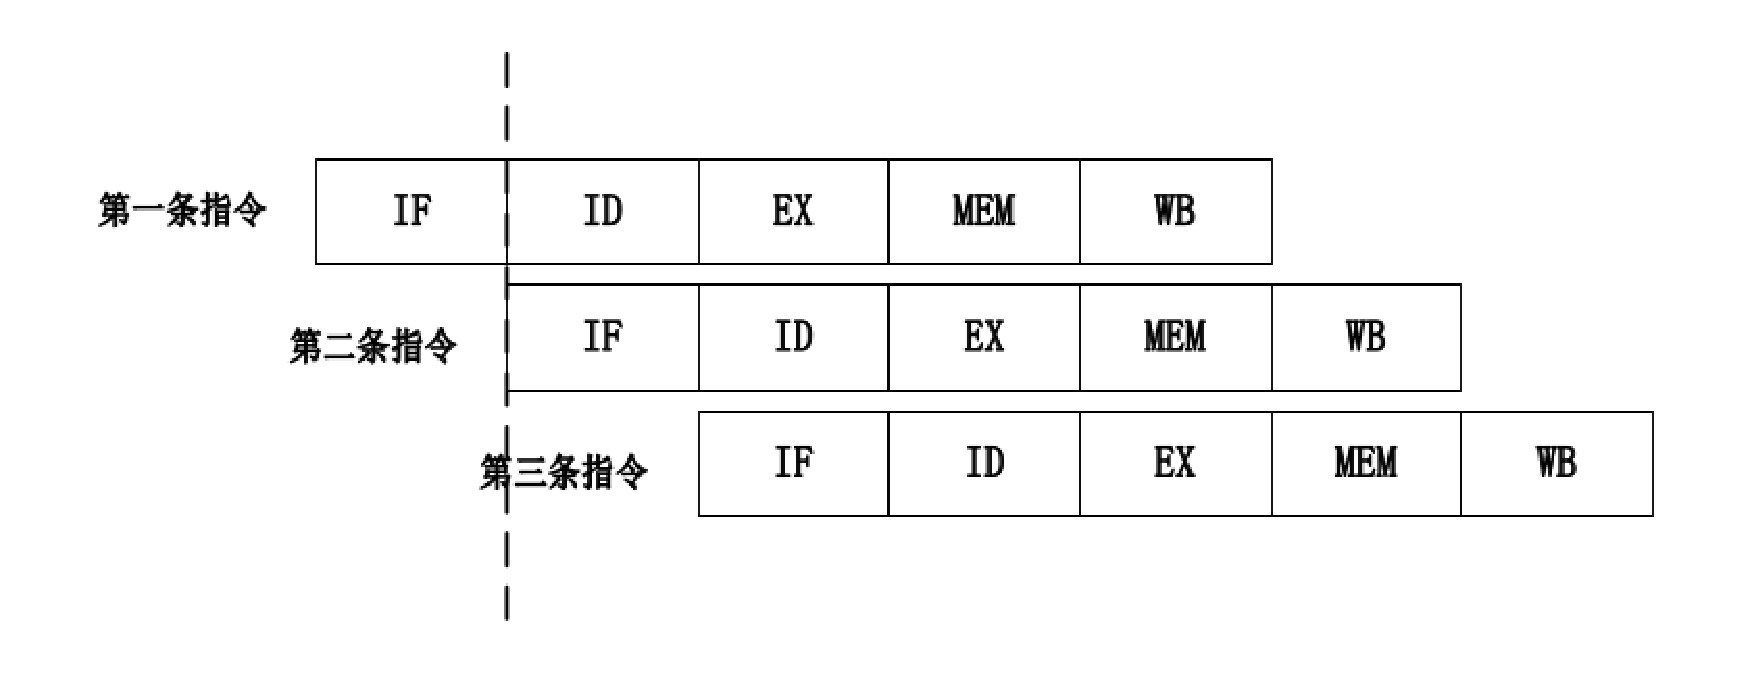
\includegraphics[width=16cm,height=9cm]{figures/chap03/cpu-pipeline}
  \caption{CPU五级流水线结构}
  \label{fig:cpu-pipeline}
\end{figure}

在此基础上,由于硬件设备的增加又产生了多发射的技术,即有多个流水线可以同时执行多条指令。这种指令间的重叠关系称为\textbf{指令级并行}\cite{Quantitative}。影响指令级并行的因素主要有:数据相关、控制相关和结构相关,这里重点介绍以下控制相关:

\textbf{控制相关}:如果两条指令中,有一条指令是转移指令,并且另一条指令是否被执行取决于该转移指令的执行结果,那么它们之间存在控制相关。

为了维护控制相关,现代CPU开发了一套基于硬件的转移推测技术,通过分支历史表(branch history table)来预测分支的转移,如果预测失败则需要重刷流水线,造成性能损失。


\subsubsection{Mesa3D立即模式绘制模式实现原理}


为了说明Mesa3D立即模式的实现原理,这里以svPerfGL的立即模式测试项为例展开分析:

\begin{lstlisting}
	glBegin(GL_TRIANGLES);
	for (i=0; i<tNumVerts; i++){
		glNormal3fv((GLfloat *)(tNorms+i));
		glColor3fv((GLfloat *)(tColors+i));
	    glVertex3fv((GLfloat *)(tVerts+i));
	}
	glEnd();
\end{lstlisting}

这里在一对glBegin和glEnd中间放入了大量的绘制命令,Mesa3D在调用glBegin时候首先会根据绘制图形样式,配置好info.mode信息,例如V\underline{ }008958\underline{ }DI\underline{ }PT\underline{ }POINTLIST、V\underline{ }008958\underline{ }DI\underline{ }PT\underline{ }TRILIST等等。接着会在VRAM上创建一个大小为VBO\underline{ }VERT\underline{ }BUFFER\underline{ }SIZE的空白VRAM空间,这里同样称为buffer0。VBO\underline{ }VERT\underline{ }BUFFER\underline{ }SIZE的默认值为1024*64。接着glBegin与glEnd中间的相关顶点数据就会通过宏函数ATTR(A, N, T, V0, V1, V2, V3)拷贝到buffer0中,当buffer0装满数据后,Mesa3D会备份边界顶点数据,然后将绘制命令发送给GPU进行渲染:

\begin{lstlisting}
r600_write_config_reg(cs, R_008958_VGT_PRIMITIVE_TYPE,
                      r600_conv_pipe_prim(info.mode));
cs->buf[cs->cdw++] = PKT3(PKT3_DRAW_INDEX_AUTO, 1, 
                          rctx->b.predicate_drawing);
cs->buf[cs->cdw++] = info.count;
cs->buf[cs->cdw++] = V_0287F0_DI_SRC_SEL_AUTO_INDEX |
                     (info.count_from_stream_output? 
                         S_0287F0_USE_OPAQUE(1) : 0);
\end{lstlisting}

之后创建新的buffer1来处理后续的顶点数据,如此反复直到glBegin和glEnd里面的数据全都装载完毕并交给GPU处理。简单来说整个过程就是如图\ref{fig:immediate-mode-flow}所示。这里与图\ref{fig:display-list-flow}里面的显示列表实现机制的不同在于显示列表机制下只需要进行一次的数据装载,以后每次调用显示列表时候就不必再数据装载了,而立即模式下每次调用都需要重新的数据装载。

\begin{figure}[H] 
  \centering
  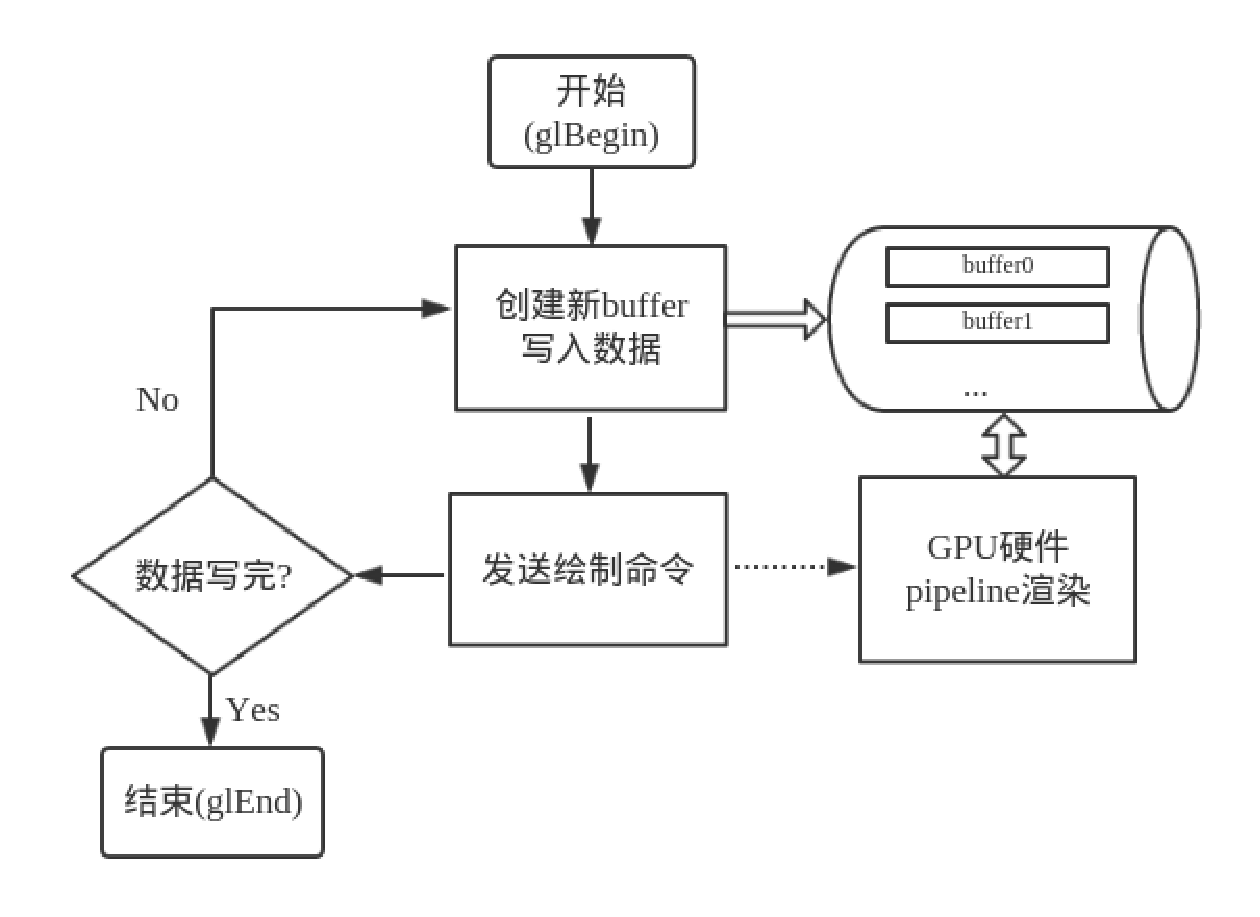
\includegraphics[width=14cm,height=10cm]{figures/chap03/immediate-mode-flow}
  \caption{Mesa3D图形库立即模式实现机制}
  \label{fig:immediate-mode-flow}
\end{figure}

\subsection{CPU端计算热点分析}

我们通过perf性能分析工具分析svPerfGL程序立即模式测试项,测试每帧绘制100万个三角形,绘制60秒后得到相关总体性能参数如下:

\begin{center} \tablecaption{svPerfGL立即模式测试项总体性能分析 \label{tab:imm-perf-stat}} 
\tablefirsthead{
\rowcolor[gray]{0.8}
\multicolumn{1}{c}{\textbf{性能参数项}} &
\multicolumn{1}{c}{\textbf{数值}} \\ }
\tablehead{\multicolumn{2}{c}{
\small 表 \ref{tab:imm-perf-stat} (续) } \\
\rowcolor[gray]{0.8}
\multicolumn{1}{c}{\textbf{性能参数项}} &
\multicolumn{1}{c}{\textbf{数值}} \\ }
\tabletail{\bottomrule
\multicolumn{2}{c}{\small 接下页} \\}
\tablelasttail{\bottomrule}

%./svPerfGL -i ../../trisNormsColors-512.nc -w 1280 -h 1024 -2 -v -t 60 -s 3000000
\begin{supertabular}{p{6.cm}p{6.cm}}
	task-clock& 114772\\
	context-switches& 1104\\
	CPU-migrations& 29\\
	page-faults& 21416\\
	cycles & 102945713309\\
	instructions& 56907962593\\
	branches& 8563703440\\
	branch-missess& 836558158\\
\end{supertabular}
\end{center}

此外,使用perf分析测试程序的热点代码后,得到占总程序一半左右的执行时间比例的热点代码段是前面章节分析提到的宏函数ATTR(具体代码参考附录\ref{cha:attr})。



% 分支预测失败率统计

\subsection{CPU端优化技术}

针对前一节的性能分析结果,本节围绕ATTR宏函数的代码特点提出了两种优化方法:

\begin{itemize}

\item{\textbf{分支结构优化}}

从性能分析表\ref{tab:imm-perf-stat}可以看出,总体的分支预测失败率较高(9.77$\%$)。具体到Mesa3D图形库热点代码ATTR宏函数\ref{cha:attr}实现来看就是以下几行代码造成的:

\begin{lstlisting}
if (N>0) dest[0] = V0;						\
if (N>1) dest[1] = V1;						\
if (N>2) dest[2] = V2;						\
if (N>3) dest[3] = V3;						\
\end{lstlisting}

因为ATTR宏函数是glVertex、glColor和glTexCoord等函数的具体实现函数,就以glVertex浮点类型为例,根据参数个数的不同OpenGL接口就定义了glVertex1f、glVertex2f、glVertex3f和glVertex4f等几种,所以上述代码里面的N就对应glVertex函数的参数个数。那么我们假设在上层应用情景中调用glVertex浮点函数时候glVertex1f、glVertex2f、glVertex3f和glVertex4f的调用频率分别为$f_1, f_2, f_3和f_4$,那么很显然有:
$$
f_1 + f_2 + f_3 + f_4 = 1
$$

由于N为1,2,3和4时候在上述代码段分别需要分支跳转判断都是4次,所以glVertex浮点函数分支跳转在执行上述代码段的平均跳转期望次数就是:

$$f_1*4 + f_2*4 + f_3*4 + f_4*4 = 4$$

这里很显然可以发现上述代码中很多判断是重叠的,比如N是否大于1这个判断是N是否大于2这个判断的真子集,即N大于2成立便可推导出N大于1,不必再进行判断。所以基于这个发现,本文改进了这个判断过程,改进后结果如下:

\begin{lstlisting}
switch(N){	\
case 4: dest[3] = V3;						\
case 3: dest[2] = V2;						\
case 2: dest[1] = V1;						\
case 1: dest[0] = V0;						\
default: \
} \
\end{lstlisting}

改进后代码跳转期望次数为:

$$f_1 * 4 + f_2 * 3 + f_3 * 2 + f_4 * 1 < 4$$

所以从根本上减少了分支跳转代码,缓解了因龙芯平台分支预测率较低带来的性能损失。

\item{\textbf{循环优化}}

除了上面分析的分支跳转的CPU端性能瓶颈以外,还存在着一些循环相关的性能瓶颈。针对这一类的瓶颈主要采用循环展开和循环化简的优化方法。

例如热点循环:
\begin{lstlisting}
for i \leftarrow 1 to n {
	memcpy(A, B, m*sizeof(typeof(A)))
	A \leftarrow A + m;
	B \leftarrow B + m;
}
}
\end{lstlisting}
这个循环就可以直接进行进行循环化简,变成memcpy(A, B, n*m*sizeof(A)),这样做的好处在于减少了glibc库函数memcpy的调用次数,优化之前需要调用n次,优化后只需要调用一次,减少了函数调用的开销。

其他的例如一些宏函数,由于编译器的保守原因,对宏函数里面的循环展开不够,例如ATTR里面的for循环就可以采用循环展开优化性能。

\item{\textbf{MIPS64编译优化}} \\
由于龙芯平台的历史发展原因,很多MIPS32\cite{Mips}的指令的硬件支持不够,譬如sqrt指令都是通过大量的运算指令软件模拟实现的,而后来随着硬件的发展和编译器的优化,龙芯发展出了MIPS64指令集,该指令集硬件支持更好,编译器编译出的汇编指令执行效率更高,所以龙芯3A平台Mesa3D库采用MIPS64编译优化以提高CPU端的计算性能。


\end{itemize}
